\chapter{BACKGROUND AND RELATED WORK}

In this chapter, we review some of the associated
topics which are pertinent to the research
performed in this dissertation. Accordingly, we
present background and related work in the areas of
wireless sensor networks (WSN) middleware, resource
management in WSN and sparse WSN. We also provide a
brief introduction to reinforcement learning (RL),
multi-agent systems and collective intelligence
(COIN) theory which plays significant role in our
work.

\section{Wireless Sensor Networks Middleware}

Complexity of sensor network applications is
continuously increasing with the proliferation of
distributed computing and wireless connectivity in
sensor networks. Heterogeneity of sensor networks
in terms of hardware characteristics as well as
application requirements further adds on
application complexity. As a result, developing
sensor network applications has become very
difficult. A middleware infrastructure is required
which can ease up scuh application development.
Challenges faced by WSN applications and
requirement and design principles of a middleware
emerging out of those challenges are discussed
next.

\subsection{WSN Middleware Challenges} Development
and implementation of a sensor network middleware
is not a trivial task and the main reason for this
is some inherent characteristics of wireless sensor
networks. We have tried to capture some of these
characteristics here. \begin{itemize} \item Sensor
nodes are limited in amount of energy they can
store or achieve from the environment. This size
and energy limit implies extremely resource
constrained devices in terms of CPU power, memory
and wireless bandwidth and range which in turn
limits processing and interactions normally
required by distributed systems. \item Sensor nodes
are subject to failures more regularly either due
to depletion of battery or environmental
influences. Also nodes can be highly mobile. this
brigns in high degree of dynamics and uncertainty
in WSN and can result in frequent topology changes
and network partitions. \item Wireless link used by
low power sensor nodes is also normally error
prone. Hence communication failure is also a
problem to be addressed. \item WSN is often
heterogeneous, e.g. a network often consists of
nodes/devices with various capabilities in terms of
sensors, computing power and memory. This further
complicates WSN management. \item A WSN application
consisting of hundreds or even thousands of sensor
nodes is normal and hence scalability is a major
issue here. \item Large number of sensor nodes and
possibility of their deployment in hostile or
in-accessible area mandates that such a system
provides \quote{exception-free unattended
operation} \cite{Estrin99}. This suggests the
necessity of autonomous adaptation in terms of
re-programmability and task dynamics. \item Concern
for security and privacy is more aggravated for WSN
applications because of sensitiveness of data
collected and lack of resources. \item With the
pervasiveness of sensor network applications, it
will become necessary to support multiple
heterogeneous applications with different
requirements on top of single network.
\end{itemize}

\subsection{WSN Middleware Requirements} Above
challenges can be interpreted to frame a list of
requirements for WSN middleware. This list is as
follows: \begin{itemize} \item Middleware system
should support high level abstraction hiding
complexity of dealing with individual node and
provide a holistic view of the
  network. Middleware should multiple programming
  paradigms like publish-subscribe, pull-push
  models, event based etc. \item It is necessary
  for WSN middleware to be very efficient in terms
  of energy, bandwidth and computational resources
  consumption. \item Middleware should be proactive
  and support adaptive fidelity algorithms to
  improve performance. \item Middleware should be
  able to provide support for programmability i.e.
  deployment, configuration and reconfiguration. It
  should also provide mechanisms for application
  policy creation and distribution. \item WSN
  middleware needs to provide scalability in terms
  of number of sensor nodes, applications running
  on top of it and associated users. \item
  Middleware needs to support execution of multiple
  applications simultaneously on a single sensor
  network. It should be able to support QoS
  requirements of individual application in terms
  of availability, timeliness, fault-tolerance etc.
  \item WSN middleware should be able to provide
  optimal network configurations in order to
  support high degree of dynamics of WSN. \item It
  should provide security in context of data
  processing, data communications, device tampering
  etc. \item Finally, middleware itself should be
  lightweight in terms of computation and
  communciation requirements
in order to be successful in resource constraint
wireless sensor networks. \end{itemize}

\subsection{WSN Middleware Design Principles} Based
on some previous work \cite{Estrin99,Yu04}, we have
hereby listed some design principles to aid in
design of middleware fulfilling above requirements.
\begin{itemize} \item A WSN middleware framework
should support the data-centric or data-driven
model for data processing and querying. \item A WSN
middleware should allow incorporation of
application knowledge and hence allow overall
software to be tailored to the executing
application. This conflicts with desire to support
and optimize for a wide class of applications.
Hence a trade-off is required between application
specification and generality of the middleware.
This is most of the time resolved by allowing
application to put its unique features as code or
specification which can be interpreted by
middleware. \item Cluster-based localized
algorithms should be used for efficiently
coordinating local interactions between sensor
nodes in order to achieve global goals. This can
help in creating more scalable applications and can
improve robustness and efficiency in resource
utilization. \item Middleware should should support
various \emph{data reduction techniques} required
for colection and processing of sensory data.
Complex sensing tasks often require that data
collected at many nodes be fused to obtain a
high-level sensing result. For reducing
communication and energy overhead, it is necessary
to process sensory data at source to extract
relevant features. Middleware will require means to
specify application knowledge and ways to inject
this knowledge into the nodes of the network. \item
Sensor networks are mostly connected to external
background infrastructures mainly for tasking the
sensor network, as well as for evaluation and
storage of sensing results and also may provide
computing and storage resources not available to
sensor networks. Hence, middleware should allow the
integration with such background infrastructures,
providing a homogeneous view of the entire system.
\end{itemize}

\subsection{WSN Middleware Classification}

\begin{figure}[tbp]
\centerline{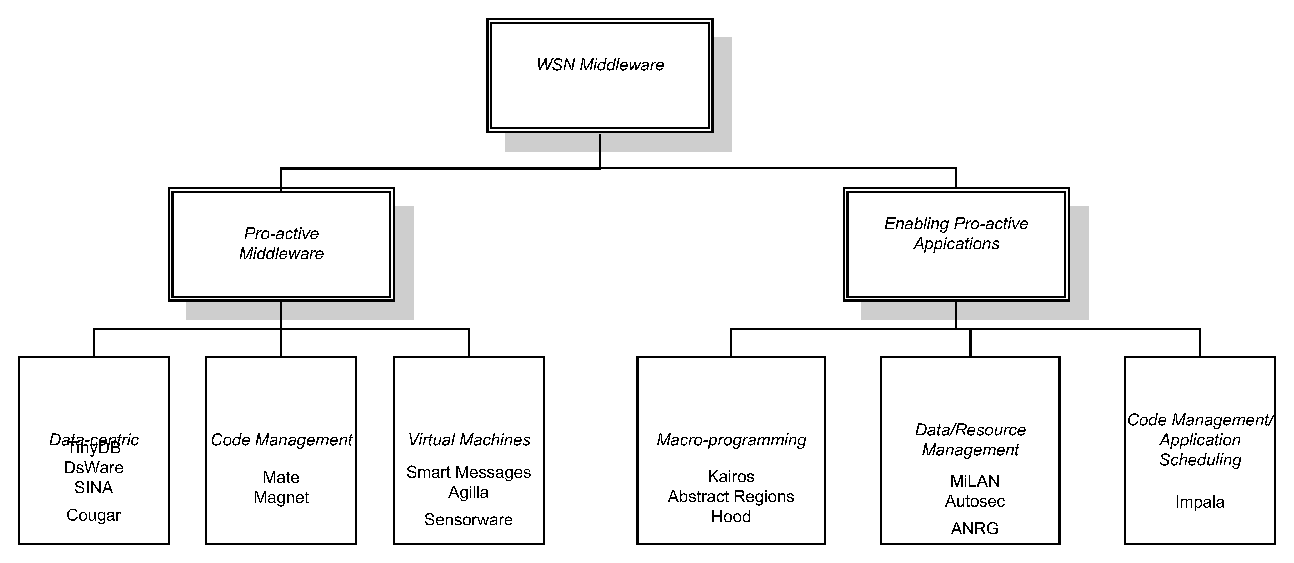
\includegraphics[width=4in]{figures/middleware-classification.eps}}
\caption{WSN Middleware Classification}
\label{fig:middleware-classification}
\end{figure}

A high level classification of the WSN middleware
frameworks is given in Figure
\ref{fig:middleware-classification}. As shown in
the figure, WSN middleware can be broadly
classified into pro-active middleware and
middleware enabling pro-active applications
\cite{Heinzelman04}. Pro-active middleware refers
to middleware that pro-actively changes WSN
functionality based on current environment and
state of the system. On the other side, middleware
enabling pro-active applications allows application
to guide system on how to adapt to changes in the
environment and state of the system.

Pro-active middleware can be further classified
into the following:
\begin{itemize}
  \item \emph{Data-centric}: Middleware in this category provides the abstraction of the whole sensor network as a virtual distributed database. Idea is to enable utilization of higher level declarative programming language/interface upon the distributed nodes without having to deal with the network issues. User dispatches queries using some easy-to-use interface to extract data of interest. The main focus of this type of middleware is on efficient evaluation of query plans using in-network query processing. Such middleware normally only uses predefined static task schedules and normally doesn't handle adaptive task/resource management. Also the approach provides only approximate values and lacks support for real-time applications that need spatio-temporal relationships between events \cite{Hadem06}.This type of middleware are not expressive enough to implement arbitrary distributed algorithms. Cougar \cite{Yao02} is the first work considering WSN as a database. TinyDB \cite{Madden02} hides the complexity of TinyOS by building query-processing system on top of it. TinyDB allows users to extract data of interest of the sensor nodes using a SQL-like interface. SINA \cite{Srisathapornphat01} and DsWare\cite{Son03} are other two approaches falling into this category of middleware using database abstraction.
  \item \emph{Virtual machine}:These middleware abstract WSN as a collection of code interpreters that take care of running programs and scripts. Examples include
  Mate \cite{Levis02}, MagnetOS \cite{Barr02} etc. Mate is a tiny, efficient virtual machine designed and implemented on top of TinyOS \cite{TiynOS}. Mate devices code
  into small capsules of instructions. It defines and implements several frequently used functionalities and provides a single instruction API for implementing them.
  Thus Mate allows application developer to write efficient programs with minimal number of instructions. It provides a (viral) broadcast solution for propagation of
  programs broken into small capsules. MagnetOS is a power-aware operating system that provides single system image of ad hoc networks so that whole network appear as a single, unified Java VM. To achieve performance efficienty, MagnetOS supports object migration to move objects closer to data sources and hence does support code management.
  \item \emph{Code Management}: This category includes middleware solutions concentrating on providing services for code deployment including allocation and migration of code to sensor nodes. Code allocation includes initial sensor selection for code execution. Code migration involves transferring of code from one node to another effectively allowing to re-task the network. Middleware's efficiency relies on strategies for migrating code to sensor nodes in vicinity of
  phenomenon of interest. Generally, this type of middleware are built on top of a virtual machine that allows remote code execution and migration. They normally
  handle a trade-off between complexity of the interpreter running on the nodes and complexity of mobile node \cite{Wang08}. Task migration mainly uses mobile code (or mobile agents) moving the code to data sources to allow local data processing. Agilla \cite{Fok09} is an example of mobile-agent based middleware concentrating
  mainly on code management aspects. Sensorware \cite{Boulis07} uses TCL scripts as mobile code that gets transfered through the system to facilitate migration.
  Middleware of this type suffers from the following issues: 1) Complexity of specification and application development, 2) High resource consumption in terms of
  computation and communication costs for code migration.
\end{itemize}
%
Even though most of above middleware approaches has some support for changing WSN functionality based on system state, they do not allow application to change system behavior directly. Next we classify middleware that allow applications to adapt to current system state and environment.
\begin{itemize}
  \item \emph{Macro-programming}:Macro-programming involves programming the sensor network as a whole rather then implementing low-level software for individual nodes. The nodal behavior is automatically generated from high-level global program. This relieves developers from dealing with low-level concerns like distributed code generation, remote data access and management and inter-node program flow coordination at each network node \cite{Gummadi05,Welsh04}. Middleware in this category normally use a concept of neighborhood to allow development of localized algorithms. As nodal behaviors are automatically generated, such middleware providing system level abstraction is easier to use. But they do suffer from high communication and computational overhead with less flexibility in implementation of energy efficient algorithms as compared to programming individual nodes. Kairos\cite{Gummadi05} focuses on providing the necessary notions and concepts to design, develop, and implement a macroprogramming model on WSN. Kairos enables programmers to choose either tight or loose synchronization based on their needs. Abstract Regions\cite{Welsh04} provide a suite of general purpose communication primitives for WSN that handles addressing, in-network data aggregation and data sharing among network's local regions. It aims at achieving energy efficiency by reducing radio  communication with use of higher localized computation. Hood\cite{Whitehouse04} also uses local neighborhood concept similar to Abstract Regions. Hood shows that local behaviors can be implemented adequately by using neighborhood abstraction.
  \item \emph{Code Management/Application Scheduling}: Impala \cite{Liu03} is an example of a middleware enabling pro-active applications with focus on code management and application scheduling. The principal goal of Impala is to allow reliable and adaptive code management and code upgrades for long-running WSN applications with infrequent code updates. Impala is designed for Zebranet project providing wildlife tracking technology. Impala is built on top of an event-based programming model. As for adaptation, it provides a mechanism for dynamically querying operating parameters and checking them against a set of application specified rules to determine if an application switch is required. Application switching is based on a finite state machine model, where transitions are defined in the form of heuristics, and can cope with device failures. However, Impala has been specifically targeted to scenarios where all nodes are mobile and act as peers. Also Impala is being destined to run onlinux based hand-held pocket PCs and hence haslimited applications.
  \item \emph{Data/Resource Management}:Middleware solutions in this category advocate need for pro-active adaptation of resources. They handle trade-off between applications QoS requirements and WSN resources. They allow applications to affect WSN resources by varying settings over time to meet applications' goal.\\
  MiLAN \cite{Heinzelman04} (Middleware Linking Applications and Networks) focuses on a cross-layer architecture that extends into the network protocol stack and allows application to change the network. MiLAN obtains QoS requirements and sensor configurations from the application in the form of specialized graphs, monitors network conditions and based on requirements varies sensor and network configurations to optimize resource utilization and maximize network lifetime. From the specialized graphs, MiLAN determines application feasible set ($F_A$) each element of which is a set of sensors that can satisfy QoS requirements of each application specified variable. MiLAN's network plugin next chooses a network feasible set ($F_N$) that can be supported by the network based on network properties and current state. $F_A$ and $F_N$ is next combined to derive overall feasible set $F$, i.e. $F=F_A \cap F_N$. \\A cluster-based architecture is described in \cite{Yu04} using virtual-machine abstraction to separate application semantics from underlying physical infrastructure. In this framework, each cluster consisting of a set of spatially adjacent sensor nodes around target phenomena forms a basic functional unit. The framework consisted of two layers 1) resource management layer-residing only at cluster head and 2) cluster layer distributed among sensor nodes. The cluster layer is responsible for forming a cluster from a group of sensor nodes and then distribution of commands issues from cluster head into the cluster. The resource management layer is responsible for allocation and adaptation of resources so that application's QoS requirements can be satisfied. Thus all nodes in a cluster cooperate together to create an adaptive resource management layer. TinyCubus \cite{Marron05} is also an adaptive cross-layer framework for TinyOS based sensor networks. TinyCubus consists of a configuration engine that distribute components to sensor nodes based on their role and install components dynamically, and a data management framework that aims at providing adaptation of system and data management components at runtime based on application requirements and system parameters.   
\end{itemize}

Even though the issue of enabling adaptive resource management for WSN applications is addressed by some mentioned middleware solutions, they require a complete knowledge of the system. Adaptation at runtime, for most of them, is very expensive in terms of resource requirements. Most of the approaches required a centralized control to make adaptation decisions and effect global system behavior. Adaptation by code management on individual sensor nodes is very resource intensive and fragile. Such centralized system for resource management and hence will not scale with network size. Also task scheduling over individual sensor node is most of the time not addressed. We have focused on adaptive data/resource management problem for design of our WSN middleware solution and hence our work (DReL- Distributed Reinforcement Learning framework) falls in the category of \emph{Data/Resource Management} as shown in figure \ref{fig:middleware-classification}. We have used a reinforcement learning based bottom-up approach which is inherently distributed, autonomous and adaptive to dynamic changes prevailing in WSN. Rest of the chapters in this dissertation provides detailed description of our middleware framework. 

%%%%%%%%%%%%%
%%
\section{Resource Management in Wireless Sensor Networks}
In this section we provide related work focusing on resource management problem in WSN. These work can be divided into the following categories: 
\begin{itemize}
  \item \emph{Rule/Predicate logic based} \cite{Frank05,Liu03,Terfloth06}: Here a set of rules are pre-programmed on individual nodes. A rule is fired if all conditions/parameters included in rule predicate evaluates true and this may result in task adaptation. This is a simple technique but requires that all state conditions be known in advance, when adaptation might be necessary. Also it can get very complex with large number of nodes and high dynamics, when the system state is changing at a high rate. Also the effect of rule based adaptation at local sensor nodes on global WSN system/application is not considered. Generic Role Assignment (GRA) scheme \cite{Frank05} considers sensor nodes in WSN system taking on certain role in the network based on their properties such that requirements of a given role is satisfied. GRA uses rules to encode node behavior and implements an algorithm to specify a set of roles that a node can assign to itself depending on its local and neighboring node's state. GRA provides abstraction to allow specification of roles and rules for their assignment using a configuration language. Impala \cite{Liu03} uses rules to implement it's application adaptor component. Application adaptor in Impala follows a finite state machine where each state represents an application and transition between states is governed by rules represented as parametric expressions. A transition is made from one application to another if that rule satisfies. Adaptor also maintains a set of application system parameters to check for transition rules. FACTS \cite{Terfloth06} uses abstraction of facts, rules and functions for their middleware architecture where all information ranging from sensor readings to state variables is represented as facts. These facts are stored in a fact repository and processed by rules. Facts, rules and functions are local to each node of the sensor network and each node runs its own rule engine. Facts are also used as medium of information transmission across nodes.           
  \item \emph{Constraint-satisfaction based} \cite{Kogekar04, Krishnamachari03, Modi05}: Here, the problem is defined in terms of constraint-satisfaction and sometimes it is reduced to linear programming with objective function consisting of optimization parameters under given constraints (application requirements). Due to the complexity of the system, it is not always possible to reduce our resource adaptation problem into a linear programming problem without making unreasonable assumptions. Also it doesn�t always allow the distribution making it impractical in large scale WSNs. A constraint-guided software reconfiguration approach is proposed in \cite{Kogekar04} where adaptation is performed by updating software components on TinyOS motes based on constraints. Here system parameters are expressed as formal constraints on QoS parameters that are measured at runtime. Each mote monitors its local QoS parameters and transmit them to the base station. Base station components utilizes these parameters to decide whether an adaptation is necessary or not. If adaptation is required, QoS parameters along with associated constraints are fed to their model generator to finally output a new software configuration for affected motes, which is then pushed down to those motes. Krishnamachari et el. \cite{Krishnamachari03} modeled various configuration tasks of multi-hop wireless networks as distributed constraint specification problems. These configuration tasks include partitioning network into coordinating cliques, hamiltonian cycle formation and conflict-free channel scheduling. Authors mapped out the connection between critical power thresholds in wireless networks and the work on constraint satisfaction and show that the average problem complexity can be reduced by tuning the transmission power of individual nodes. A distributed constraint optimization algorithm called \emph{Adopt} \cite{Modi05} is proposed for general multi-agent systems. Modi et el. proposes a systematic formalization of the distributed resource allocation problem and a general solution strategy that maps a formal model of resource allocation into a problem solving paradigm called distributed constraint-based reasoning. Adopt uses localized asynchronous communication and makes local decisions based on conservative cost estimates rather than global certainty which results in polynomial-space algorithm.                
  \item \emph{Agent negotiation/Auction based} \cite{Lesser03, Ortiz03, Soh03}: This mainly includes multi-agent systems with agents being able to negotiate with each other in order to determine the best allocation. The system consists of one or more mediators responsible for negotiations. Although this approach can lead to efficient resource management, communication and computational resources required for these negotiations may be sometimes prohibitive for their implementation on resource constrained WSN system. A center-based algorithm called \emph{Mediation} is proposed in \cite{Ortiz03} to address task assignment problem in distributed sensor networks. Mediation implements an iterative hill-climbing search in a subset of solution space by making and sending successive proposals to group's agents. Group members provides response to the mediator based on context of the proposal and mediator uses these responses to find a satisfactory solution to the task assignment problem. Mediation algorithm is further extended to address a) changes during the decision-making process, b) negotiation over tasks whose utilities are not necessarily additive and c) monitoring and adapting a solution in non-stationary environment. A distributed resource allocation based on dynamic coalition formation and coalition strategy learning is presented in \cite{Soh03}. In this scheme, agents attempt to operate autonomously with incomplete information about their potential collaborators. Synchronization of actions across multiple agents is achieved by forming coalitions via multiple 1-to-1 negotiations. Though, because of uncertain properties of WSN, coaltions formed will be suboptimal and satisficing. To allow adaptation to environment dynamics, each agent is capable of multiple level of learning. This includes case-based learning to learn about how-to negotiate better and reinforcement learning to learn how-to form a better coalition.   
  \item \emph{Utility based} \cite{Byers02}: Here the purpose is to define a utility function mapping optimization parameter over a number of participating nodes to a real value and maximize these functions under given constraints. This can further take the form of the linear programming problem, but doesn�t allow easy distribution of task management process.
\end{itemize}  
Even though, each of the approaches mentioned above can provide efficient resource management, they suffer from some pitfalls as described. None of these techniques try to address uncertainty which is inherent in dynamic networks. Furthermore, most of them require a careful implementation of algorithms on a case-by-case basis which may be quite difficult in sensor networks. Therefore, a framework that can enable large set of applications with autonomous adaptation and minimum communication overhead is required.  
 

% Market/economics based, AI based, %
% centralized/distributed, % coin
\section{Reinforcement Learning} %Q-learning, MAS,
RL based MAS, COIN
\section{Sparse WSN}
More recently, the TinyLime [7] middleware has been proposed for the specific scenario of sparse WSNs. TinyLime is based on a tuple space model, an implementation of the distributed shared memory paradigm for distributed computing. The original tuple space model is extended to the scenario where multiple MDCs collect data from sensor nodes which are not densely deployed in the network. To this end, no assumption is made on network connectivity, since nodes can even be isolated from each other. TinyLime provides mechanisms to perform data aggregation and tune the activity of nodes in order to save energy. However, the focus of TinyLime is on their proposed programming abstraction rather than on adaptation and resource management.


